\documentclass{article}
\usepackage{color,soul}
\usepackage{amsmath}
\usepackage{amsfonts} 
\usepackage{eqnarray}
\usepackage{bm}
\usepackage{multirow}
\usepackage{graphicx}
\usepackage{booktabs}
\usepackage{comment}
\usepackage{subcaption}
\usepackage{listings}
\usepackage{pythonhighlight}
\usepackage[margin=0.5in]{geometry}

\title{School of Electrical and Computer Engineering\\
Purdue University, WL, IN, USA}
\author{Nahian Ibn Hasan\\
Email: hasan34@purdue.edu\\
PUID: 0032764564\\
ECE66100 - Computer Vission\\
Fall 2022\\
Homework-10}
\date{\today}

\begin{document}
\maketitle
\section{Objective}
The goal of this homework is to apply principal component analysis (PCA), linear discriminant analysis (LDA), autoencoder and cascaded AdaBoost algorithm for image classification.
\section{Principal Component Analysis (PCA)}
The general theory ( and also the implementation process) of PCA is described step by step in the following description-
\begin{itemize}
\item For N vectorized images {$\vec{x}_i;i=1,2,3,\cdots N$}, the mean $\vec{m}$ is calculated as
\begin{equation}
\vec{m} = \frac{1}{N}\sum_{i=1}^{N}\vec{x}_i
\end{equation}
\item The covariance of the dataset is calculated with the following expression-
\begin{equation}
C = \frac{1}{N}\sum_{i=1}^N\{(\vec{x}_i-\vec{m})(\vec{x}_i-\vec{m})^T\}
\end{equation}
If the image vectors $\vec{x}_i$ (flattened from 2D image to 1D vector) are of dimension $n$, then with the above covariance formula, the covariance matrix (C) will be of size $n\times n$. Therefore, an alternative approach is to construct a zero-mean matrix $X$ as follows-
\begin{equation}
X = [\vec{x}_1-\vec{m} | \vec{x}_2-\vec{m} | \cdots |\vec{x}_N-\vec{m}]
\end{equation}
From the above covariance formula, it can be shown that,
\begin{equation}
	C = XX^T
\end{equation}
However, since, C is of large size, in subsequent steps of PCA, it's computationally expensive to calculate eigenvectors, hence, we calculate modified eigenvectors  of the smaller matrix 
\begin{equation}
	C = X^TX
\end{equation}
Later, the actual eigenvectors can be calculated, which is described in the next steps. The data are being normalized columnwise for computational efficiency.
\item The eigenvectors of the matrix C are calculated and the $P$ eigenvectors corresponding to the highest $P$ singular values are retained. Say, $U_P$ denotes the set of eigenvectors retained as separate columns, where
\begin{equation}
	U_P = [\vec{u}_1 | \vec{u}_2 | \vec{u}_3 | \cdots | \vec{u}_P]
\end{equation}
\item Since, we need to find out the actual eigen vectors, the actual eigen vectors ($W_P$) are
\begin{equation}
	W_P = XU_P
\end{equation}
\item Since, the images are real, the real part of the eigen values are considered for further processing. Also, the eigen vectors are normalized -
\begin{equation}
	\vec{\hat{w_i}} = \frac{\vec{w}_i}{||\vec{w}_i||}
\end{equation}
\item The data are projected to this $P$ dimensional  space as follows-
\begin{equation}
\vec{y} = \hat{W}_P^T(\vec{x} - \vec{m}).
\end{equation}
Here, $\vec{y}$ is $P$ dimensional.
\item In this way, for every image in the dataset, there is a $P$-dimensional vector representation which denotes a low-dimensional projection of the original image. Usually $P<<n$.
\item A nearest neighbour (NN) classification has been implemented for this assignment to classify the images based on the projected $P$-dimensional vectors using the Euclidean L2 norm as the distance metric between the ground truth and predicted images.
\item For this assignment, the number of nearest neighbours is assigned as 1 and the classification results for $P=1\cdots 25$ are shown. Number of classes is $30$. There are $21$ image samples within each class. The database is consists of human faces.
\end{itemize}
\section{Linear Discriminant Analysis (LDA)}
LDA is an alternate approach for dimentionality reduction like PCA. PCA seeks an orthogonal set of maximal-variance directions in the underlying vector space for all training data whereas LDA seeks the dimensions in the underlying space that maximally discriminates between classes. A maximally discriminating vector simultaneously maximizes the between-class scatter and minimizes the within-class scatter. The step-by-step process of the LDA is described here-
\begin{itemize}
\item Say, the image set corresponding to class $i$ is denoted as $C_i$ and $C$ denotes the set of all images. Moreover, $|C_i|$ and $|C|$ denote the number of image samples in class $i$ and number of total images in the whole dataset, respectively. The mean corresponding to class $i$ is 
\begin{equation}
	\vec{m_i} = \frac{1}{|C_i|}\sum_{k=1}^{|C_i|}\vec{x}_{k}^i
\end{equation}
and the global mean of all images is 
\begin{equation}
	\vec{m} = \frac{1}{|C|}\sum_{k=1}^{N}x_k.
\end{equation}
Here, $N$ is the total number of images in the whole dataset.
\item The between-class scatter matrix is defined as
\begin{equation}
	S_B = \frac{1}{|C|}\sum_{i=1}^{|C|}\{(\vec{m}_i-\vec{m})(\vec{m}_i-\vec{m})^T\}
\end{equation}
If each image is vectorized (flattened) to a vector of size $n$, the dimension of the matrix $S_B$ is $n\times n$.
\item The within-class scatter matrix is defined as 
\begin{equation}
	S_W = \frac{1}{|C|}\sum_{i=1}^{|C|}\frac{1}{|C_i|}\sum_{k=1}^{|C_i|}\{(\vec{x}_k^i-\vec{m}_i)(\vec{x}_k^i-\vec{m}_i)^T\}
\end{equation}
here, $\vec{x}_k^i$ is the $k^{th}$ image of $i^{th}$ class. Similar to $S_B$, $S_W$ is also of size $n\times n$.
\item We want to minimze the Fisher Discriminant Function ($J(\vec{w})$) for any vector $\vec{w}$, where
\begin{equation}
	J(\vec{w}) = \frac{\vec{w}^TS_B\vec{w}}{\vec{w}^TS_W\vec{w}}.
\end{equation}
This boils down to finding the few eigenvectors corresponding to the largest few eigenvalues of the matrix  $S_W^{-1}S_B$.
\item There is a high probability that $S_W$ is either singular or close to siingular. Therefore, we utilizea slight variant of the original LDA approach which has been proposed by Yu and Yang [3]. According to this modified approach, first, we calculate the eigen vectors ($v$) of $S_B$ corresponding to its highest $K_Y$ eigenvalues. In our implementation in this report, $K_Y=11$ happens to provide a very good performance. The eigen vectors are normalized -
\begin{equation}
	\vec{\hat{v}}_i = \frac{\vec{v}_i}{||\vec{v}_i||};\;\;\;\;\hat{V} = [\vec{\hat{v}}_1 | \vec{\hat{v}}_2 | \cdots | \vec{\hat{v}}_{K_Y}]
\end{equation}
\item A low dimensional projection ($Z$) of original $S_B$ matrix is constructed with these truncated number of eigenvalues and eigenvectors.
\begin{equation}
	Z = \hat{V}D_B^{-0.5},
\end{equation}
where, $D_B$ is a diagonal matrix with the highest $K_Y$ eigenvectors along the diagonal.
\item Next, the highest eigenvectors corresponding to the highest $P$ eigenvalues of the matrix $G=Z^TS_WZ$ are extracted using eigenvalue decomposition. These eigenvectors are also normalized. Let's assume, these normalized eigenvectors are denoted as $\vec{\hat{u}}_i$ and $\hat{U} = [\vec{\hat{u}}_1 | \vec{\hat{u}}_2 | \cdots | \vec{\hat{u}}_P]$. Then the final projection matrix is formed as 
\begin{equation}
	W_P = (U^TZ^T)^T,
\end{equation}
where, each column of $W_P$ are the maximally discriminating directions.
\item Finally, a $P$-dimensional vector projection of every image can be found as
\begin{equation}
	y_i = W_P^T(\vec{\hat{x}}_i - \vec{m}).
\end{equation}
Similar to PCA in the last section, we can apply NN classifier for classifying the images. We have utilized the same database as in PCA and the number of nearest neighbour is also set to 1 like PCA analysis.
\end{itemize}
\section{Autoencoder}
An autoencoder is a type of neural network that is commonly used for dimensionality reduction. It is comprised of two neural network based components: an encoder and a decoder. The encoder takes in an high-dimensional sample such as an image and outputs a p-dimensional vector representation just like PCA and LDA. The decoder then takes in the p-dimensional vector representation and outputs a sample (e.g. an image) in the original high-dimensional sample space. During training, the autoencoder refines itself by attempting to regenerate the input sample from the corresponding p-dimensional vector representation.
\subsection*{Autoencoder Implementation Notes}
\begin{itemize}
\item[1.] A pretrained autoencoder has been tested on the dataset for $P=3,8,16$.
\item[2.] The autoencoder has been trained from scracth for $P=1,2\cdots 25$
\item[3.] The autoencoder is implemented in Pytorch. For each image, the autoendoer predicts a low-dimensional projection of length P.
\item[4.] Next, a NN classifier classifies the image.
\item[5.] The model has a decoder part as well which tries to reconstruct the image form the encoded information. During the training stage, the image is first encoded, and a reconstructed image is predicted by the decoder which is then used to calculate the variational autoencoder loss along with the ground truth image.
\item[6.] During the testng (inference) stage, The model encoder generates the encoded information and using the encoding for both trainng and testing set, the NN classifier classifies the images.
\end{itemize}

\section{Cascaded Adaboost Classifier}
A cascaded Adaboost algorithm has been implemented based on Viola and Jones approach [4]. The cascaded implementation tries to meet a target false-positive-rate (FPR) and True-detection rate. From a general overall high-level view of the algorithm, there are several weak classifiers which are cascaded together to form a very strong classifier. Each weak classifier is well enough trained to classify at least 50\% of the data. Based on a 'polarity' parameter (in other words, a thresholding direction parameter). The step-by-step process is described below-
\begin{itemize}
\item The first step is to extract low-level features of the image. For this assignment, we have chosen Haar filters to extract features from the image. The dimension of the Haar filter windows are $2,4,6,8,\cdots,(M or N)$, assuming the width and heights of the image are $M$ and $N$, respectively. We have applied the Haar filters both horizontally and vertically. An example of horizontal and vertical Haar filter are-
\begin{equation}
	\begin{bmatrix}-1 & -1 & 1 & 1\end{bmatrix}
\end{equation}
\begin{equation}
	\begin{bmatrix}-1 \\ -1 \\ 1 \\ 1\end{bmatrix}
\end{equation}
The convolution features are stored in a long vector with the horizontal features followed by vertical features.
\item The data features of all images are stored in a matrix with size ($X\times Y$), $X$ denoting the number of sample images and $Y$ denoting the feature length of each image. Also, a separat label for each feature is prepared with label='1' for positive car images and label=-1 for negative car images.
\item A weight matrix is associated with each data sample. Initially, all the weights are uniformly distributed with equal probability. The weight corresponding to any  sample dictates the probability of considering that image for training in the subsequent iterations of a cascading lavel.
\item A weak classifier is formed by first normalizing the weights. By iterating over each feature across all images, we sort the features according to the numeric value of the feature. Withing the same sorting sequence, the corresponding labels and weights are also sorted.
\item Error is calculated for different polarity separately. For example, eror of polarity 1 is calculated as $e_1 = C^+ + T^- -C^-$, where $C^+$ and $C^-$ denote the cumulative sum of all the positive and negative label's weights, respectively, which are less than the current threshold. SImilarly, error for polarity 2 is calculated  with signs in the superscript reversed in the above formula. These two errors are concatenated in a single matrix. hence, for each feature, we have two errors. We find the miimum index corresponding to the minimum value of these errors and the corresponding feature value to that index is considered the next threshold value if the minimum error is lower than the previous minimum error. The class labels are predicted based on this minimum value and the polarity is decided whether the error at the minimum index is due to error type 1 or error type 2. In this way, among all the features we find the feature that discriminates classes most effectively and that becomes the first candidate of the weak classifier in iteration 1 in cascade 1. Say, this classifier is $h_t$.
\item We calculate a trust factor ($\alpha_t$) for this classifier as follows
\begin{equation}
	\alpha_t = \frac{1}{2}ln\bigg(\frac{1-\epsilon_t}{\epsilon_t}\bigg)
\end{equation}
where,
\begin{equation}
	\epsilon_t = \frac{1}{2}\sum_{i=1}^{X}D_t(x_i).|h_t(x_i) - y_i|
\end{equation}
Also, the weights for each sample for the next iteration are updated as follows-
\begin{equation}
	D_{t+1}(x_i) = \frac{D_t(x_i)e^{-\alpha_ty_ih_t(x_i)}}{Z_t}
\end{equation}
where,
\begin{equation}
	Z_t = \sum_{i=1}^{X}D_t(x_i)e^{-\alpha_ty_ih_t(x_i)}
\end{equation}
\item Next, we start again with the new weight and the same data and labels again to hunt for a new and better candidate of the weak classifier. After N iterations, we have the best candidate to be a weak classifier for that cascade level. In some reports it has been mentioned to prediict the label of an image by considering all the weak classifier candidates and multiply their label predictions with the trust factor ($\alpha_t$). However, following some reports in the literature, in this assignment, we consider only the weak classifier that that has the best trust factor. It turns out to perform very well in terms of reducing the false positive rate in successive cascading layers.
\item Tis concludes the cascading level 1. before going to the next level, we only pass the positive images from the current cascade level since we only want to reduce the faslse positive rate in successive levels. Thereafter, with the reduced dataset, we follow the same process of finding a best weak classifier for the next cascade layer and we keep adding layers until a desired level of false positive rate is achieved.
\item A desired FPR is calculated by the formula $(FPR)^r$, where $r$ is the number of cascading layers. It's a cumulative FPR formula.
\item In the testing phase, the image is passed through each best weak classifier at each cascading layer and the label is predicted according to the threshold and polarity of that classifier. Next, the trust factor ($\alpha_t$) is multiplied to have a relative weight cotribution from each classifier to finally decide the classification label. The FPR and FNR are kept track at each cascade layer to see the performance in reducing the FPR in successive  cascading layer.
\end{itemize}


\section{Results}
\subsection{Covariance Matrices of PCA and LDA}
\begin{figure}[!htbp]
     \centering
     \captionsetup[subfigure]{labelformat=empty}
    \subcaptionbox{a}{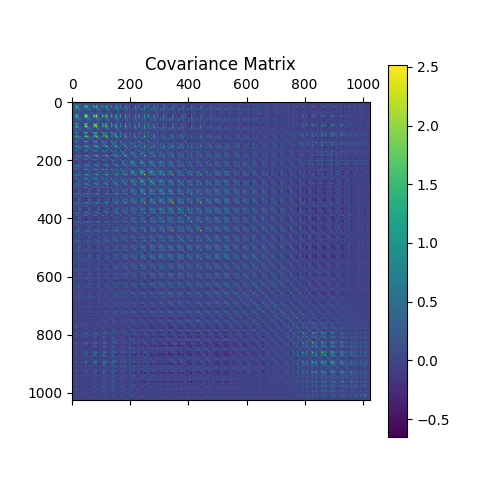
\includegraphics[width=0.32\textwidth]{../My_Code/Results/PCA/train_data_covariance_matrix.png}}
    \subcaptionbox{b}{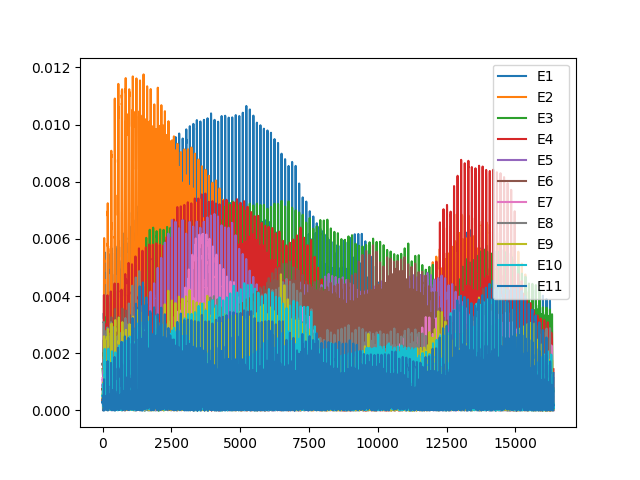
\includegraphics[width=0.45\textwidth]{../My_Code/Results/PCA/eigenvectors_K_11.png}}
    \caption{(a)Covarinace matrix for PCA (Although here, the covariance matrix is shown as $C=XX^T$, in the implementation of this assignment we utilized a reduced size of the covariance matrix by finding the eigenvectors of $C=X^TX$ and then multiplying those eigenvectors by $X$ to find out the actual eigenvectors.) (b) The eigenvectors corresponding to higest 11 eigenvalues}
    \label{fig:CM_PCA}
\end{figure}

\begin{figure}[!htbp]
     \centering
     \captionsetup[subfigure]{labelformat=empty}
    \subcaptionbox{}{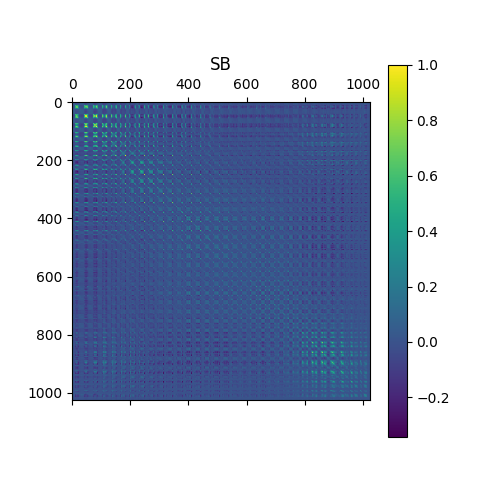
\includegraphics[width=0.32\textwidth]{../My_Code/Results/LDA/train_data_SB_yu_yang.png}}
    \subcaptionbox{}{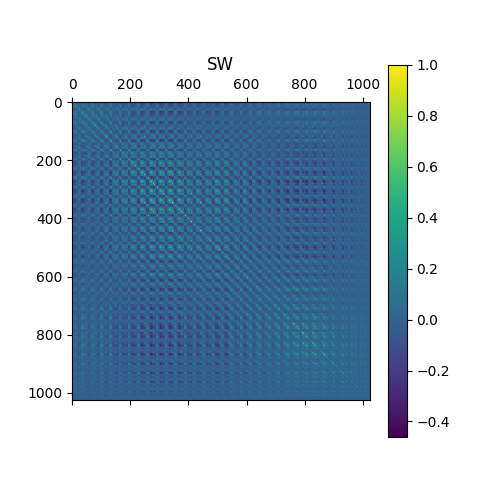
\includegraphics[width=0.32\textwidth]{../My_Code/Results/LDA/train_data_SW_yu_yang.png}}
    \subcaptionbox{}{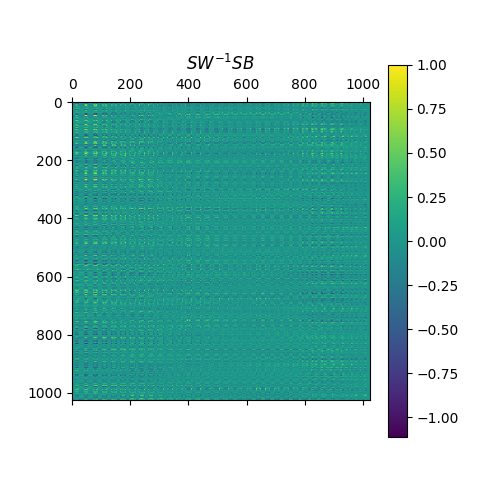
\includegraphics[width=0.32\textwidth]{../My_Code/Results/LDA/train_data_combined_scatter_matrix_yu_yang.png}}
    \caption{Between-class scatter matrix (a), within-class scatter matrix (b) and combined scatter matrix of which eigenvectors are calculated in original LDA (c).}
    \label{fig:CM_LDA}
\end{figure}

\newpage
\subsection{Eigen Faces}
The eigenvectors of the PCA covariance matrix are plotted here in the order of highest to lowest eigen values. In the literature, these images are sometimes called eigen faces. As the eigen value decreases, the corresponding eigen vectors (i.e. eigen images) become noisier. Therefore, only the highest few eigen vectors are of our importance which capture the true and necessary face features and which are enough to successfully classify images.
\begin{figure}[!htbp]
     \centering
     \captionsetup[subfigure]{labelformat=empty}
    \subcaptionbox{}{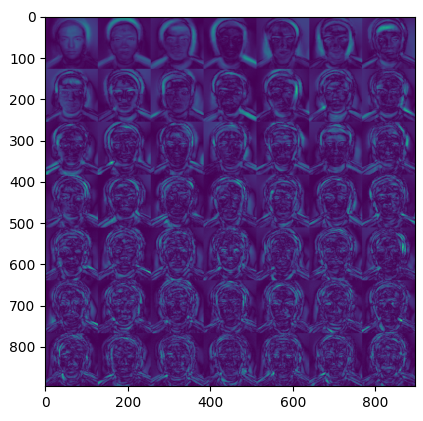
\includegraphics[width=0.99\textwidth]{../My_Code/Results/PCA/Eigen_Faces.png}}
    \caption{Eigen-Faces from PCA output. The eigen-faces are plotted in the order of highest to lowest eigen value in row-major order.}
    \label{fig:eig_face_PCA}
\end{figure}


\newpage
\subsection{Classification Accuracy Among PCA, LDA, Autoencoder (Pre-trained)}
\begin{figure}[!htbp]
     \centering
     \captionsetup[subfigure]{labelformat=empty}
    \subcaptionbox{a}{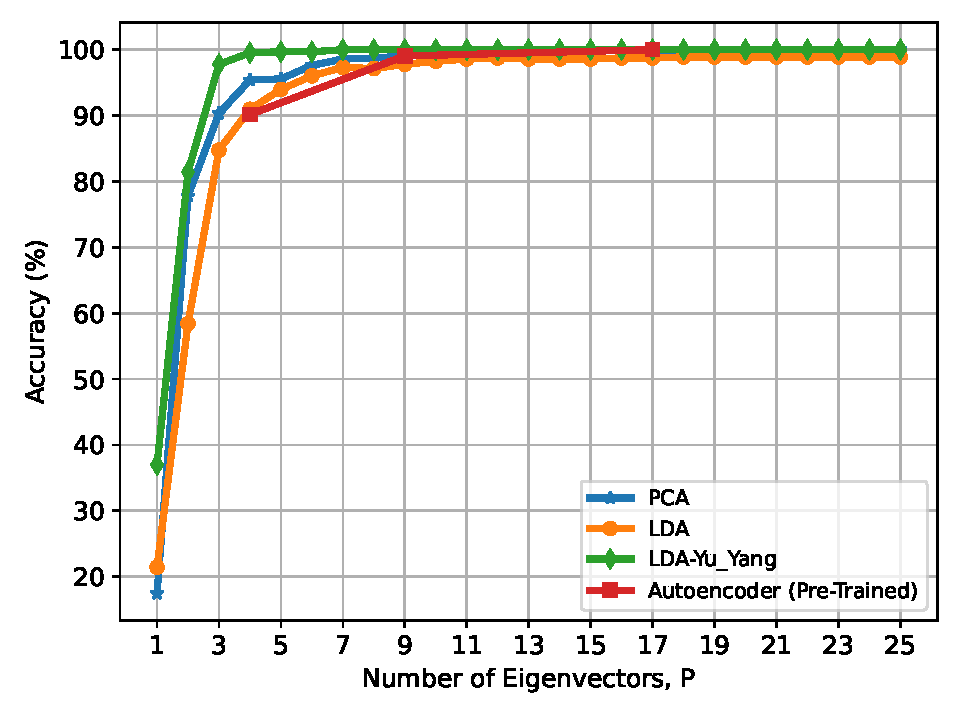
\includegraphics[width=0.44\textwidth]{../My_Code/Results/Comparison_pretrained.pdf}}
    \subcaptionbox{b}{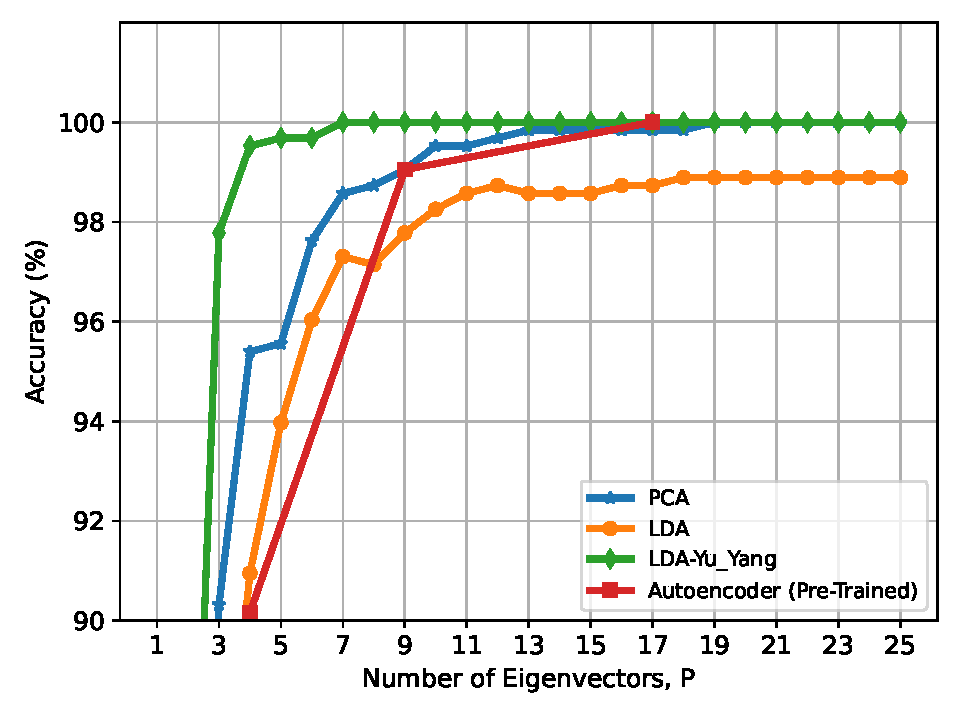
\includegraphics[width=0.44\textwidth]{../My_Code/Results/Comparison_zoomed_pretrained.pdf}}
    \caption{The comparison among the PCA, LDA (typical), LDA(Yu-Yang version) and autoencoder (pretrained) algorithm. (b) depicts a more enhanced view near optimal accuracy level.}
    \label{fig:accuracy_1}
\end{figure}

\subsection{Classification Accuracy Among PCA, LDA, Autoencoder (Custom Trained)}
\begin{figure}[!htbp]
     \centering
     \captionsetup[subfigure]{labelformat=empty}
    \subcaptionbox{a}{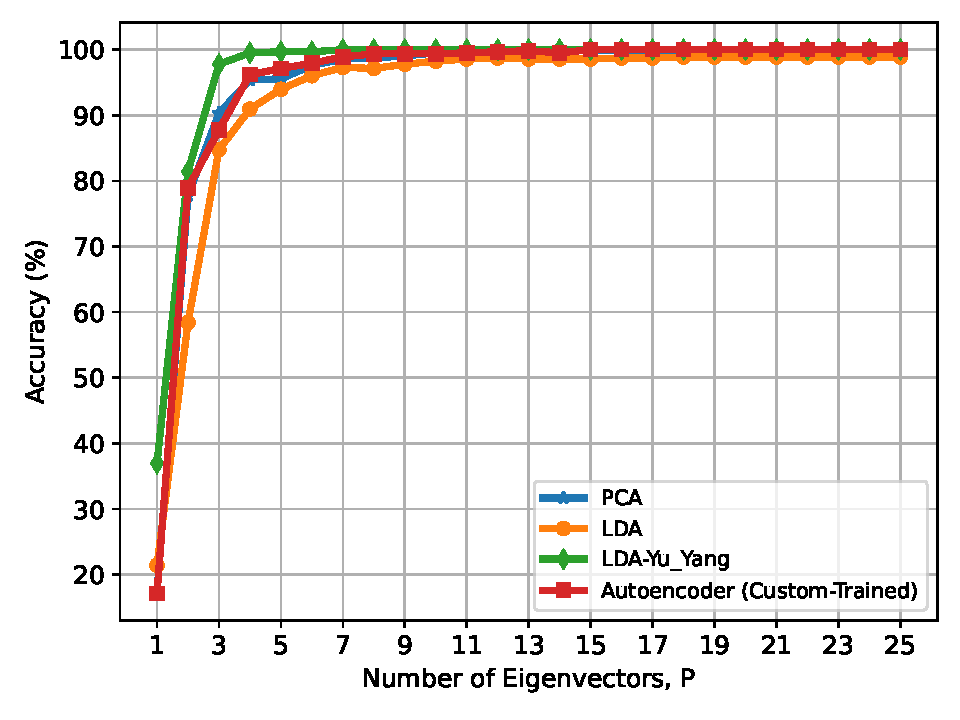
\includegraphics[width=0.43\textwidth]{../My_Code/Results/Comparison_custom.pdf}}
    \subcaptionbox{b}{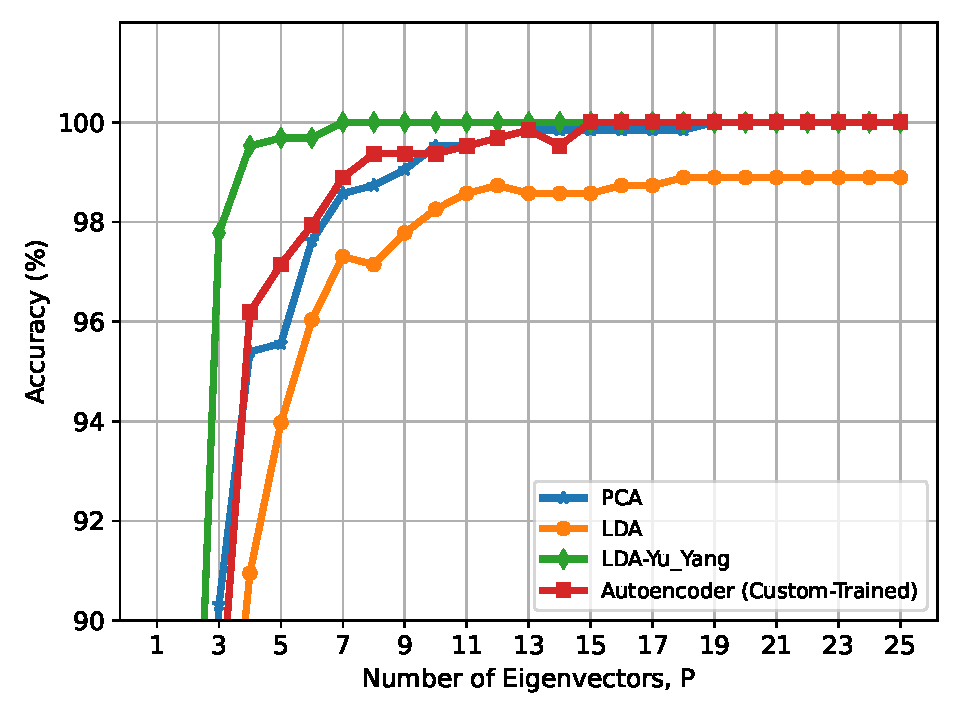
\includegraphics[width=0.43\textwidth]{../My_Code/Results/Comparison_zoomed_custom.pdf}}
    \caption{The comparison among the PCA, LDA (typical), LDA(Yu-Yang version) and autoencoder (custom trained) algorithm. (b) depicts a more enhanced view near optimal accuracy level. The autoencoder is trained from scratch to have a end-to-end comparison with other methods when the number of interest eigenvectors changes. \textbf{NB:To reproduce the autoencoder results, the model weights are attached with the source code file}.}
    \label{fig:accuracy_2}
\end{figure}
\subsection{Comments}
Fig. \ref{fig:accuracy_1} and Fig. \ref{fig:accuracy_2} show the relative accuracy of PCA, LDA and autoencoder classification. Aamong all the approaches, The LDA (Yu-Yang version) seems to be converging to optimal results much faster than other methods, followed by the autoencoder, PCA and LDA(original version), successively. The table below shows the minimum number of eigen vectors required to reach the optimal accuracy.
\begin{center}
\begin{tabular}{||c c c c||} 
 \hline
 Method & Optimum Accuracy & \# of eigenvectors to reach optimum & \# of eigenvectors to reach 99\% \\ [0.5ex] 
 \hline\hline
 PCA & 100\% & 19 & 9 \\ 
 \hline
 LDA (Original) & 98.89\% & 18 & Not-Attained \\
 \hline
 LDA (Yu-Yang) & 100\% & 7 & 4  \\
 \hline
 Autoencoder & 100\% & 15 & 8 \\
 \hline
\end{tabular}
\end{center}


\newpage
\subsection{Cascaded AdaBoost Output}
\subsubsection{Training Set}
\begin{figure}[!htbp]
     \centering
     \captionsetup[subfigure]{labelformat=empty}
    \subcaptionbox{(a)}{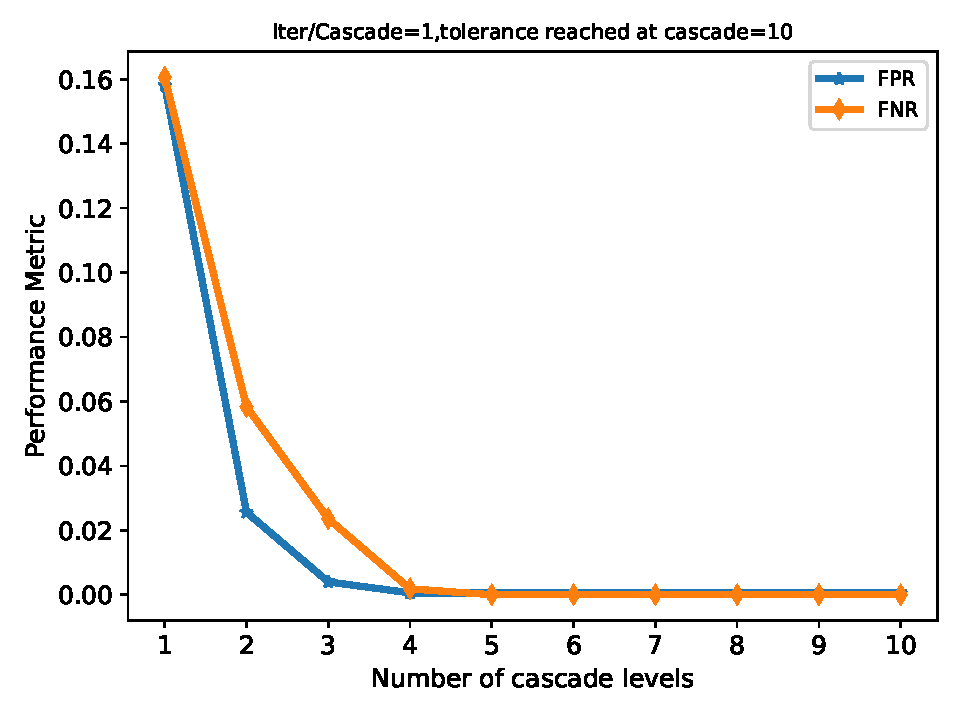
\includegraphics[width=0.32\textwidth]{../My_Code/Results/Adaboost/Adaboost_Performance_1_10_train.pdf}}
    \subcaptionbox{(b)}{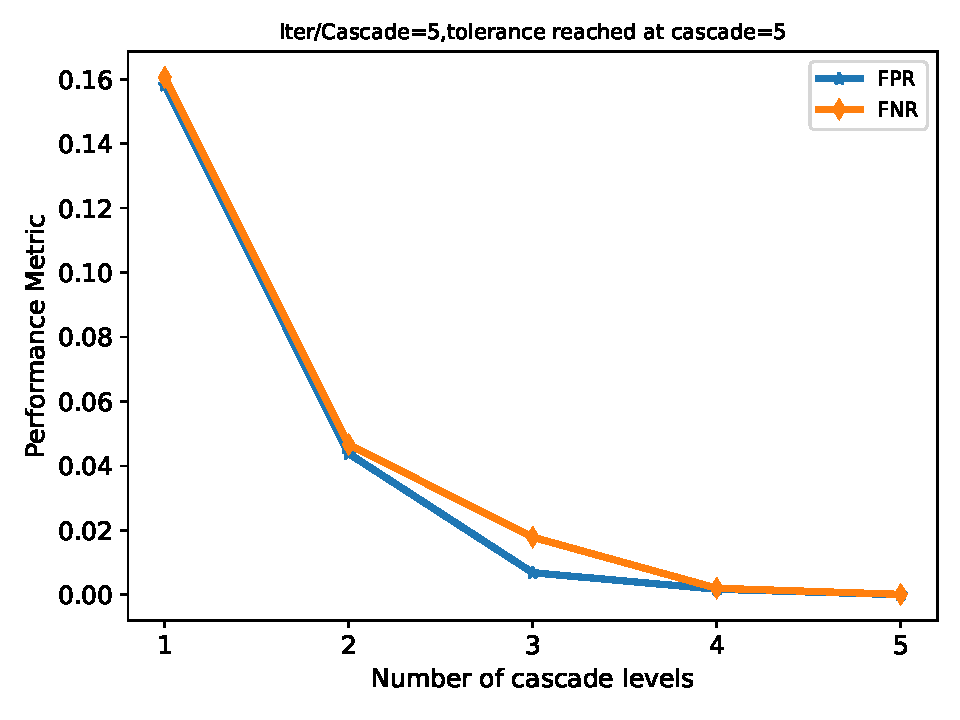
\includegraphics[width=0.32\textwidth]{../My_Code/Results/Adaboost/Adaboost_Performance_5_10_train.pdf}}
    \subcaptionbox{(c)}{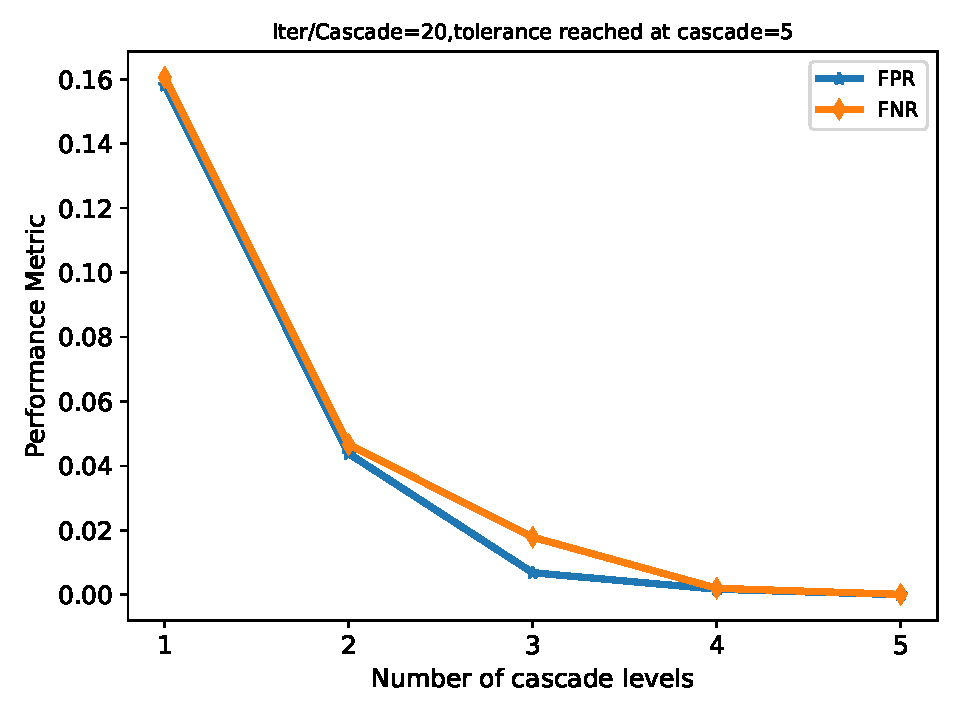
\includegraphics[width=0.32\textwidth]{../My_Code/Results/Adaboost/Adaboost_Performance_20_10_train.pdf}}
    \caption{Propagation of False Positive Rate (FPR) and False Negative Rate (FNR) at each cascading level for different number of iterations. The number of maximum cascading layers is fixed to 10. The number of iterations (N) per cascade level is set to 1 in (a), 5 in (b) and 20 in (c). The tolerance limit is set to $10^{-6}$ for FPR. It seems when N=1 in (a), the tolerance is not reached within a limit of 10 cascade levels. But for N=5 in (b) or N=20 in (c), the tolerance is reached well within 5 cascade levels. After N=5, there is not much gain in increasing N.}
    \label{fig:adaboost_1}
\end{figure}

\subsubsection{Testing Set}
\begin{figure}[!htbp]
     \centering
     \captionsetup[subfigure]{labelformat=empty}
    \subcaptionbox{(a)}{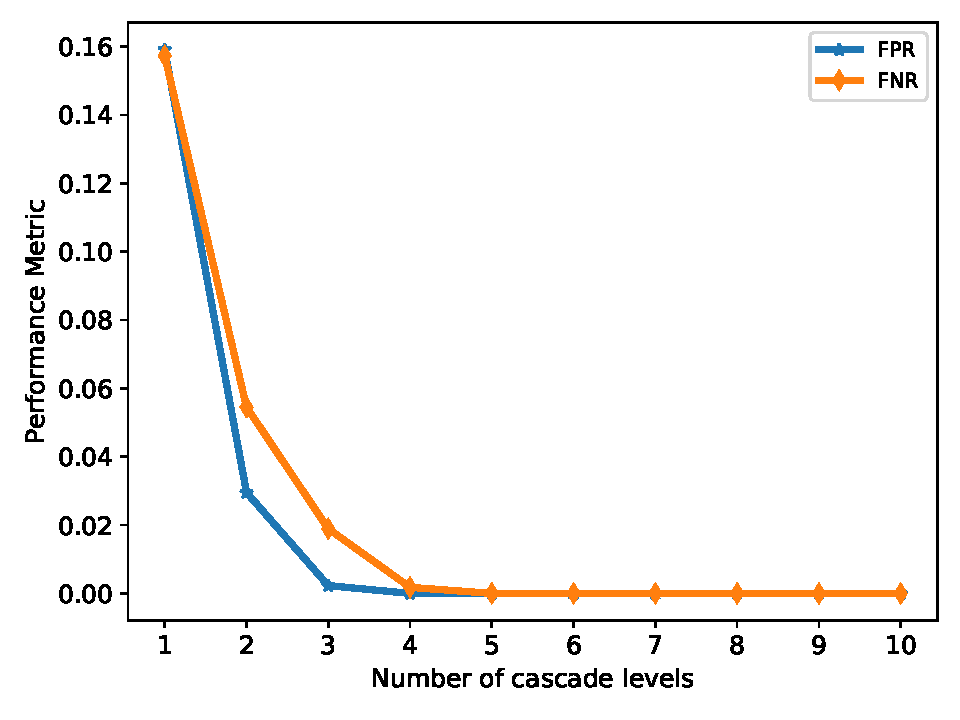
\includegraphics[width=0.32\textwidth]{../My_Code/Results/Adaboost/Adaboost_Performance_1_10_test.pdf}}
    \subcaptionbox{(b)}{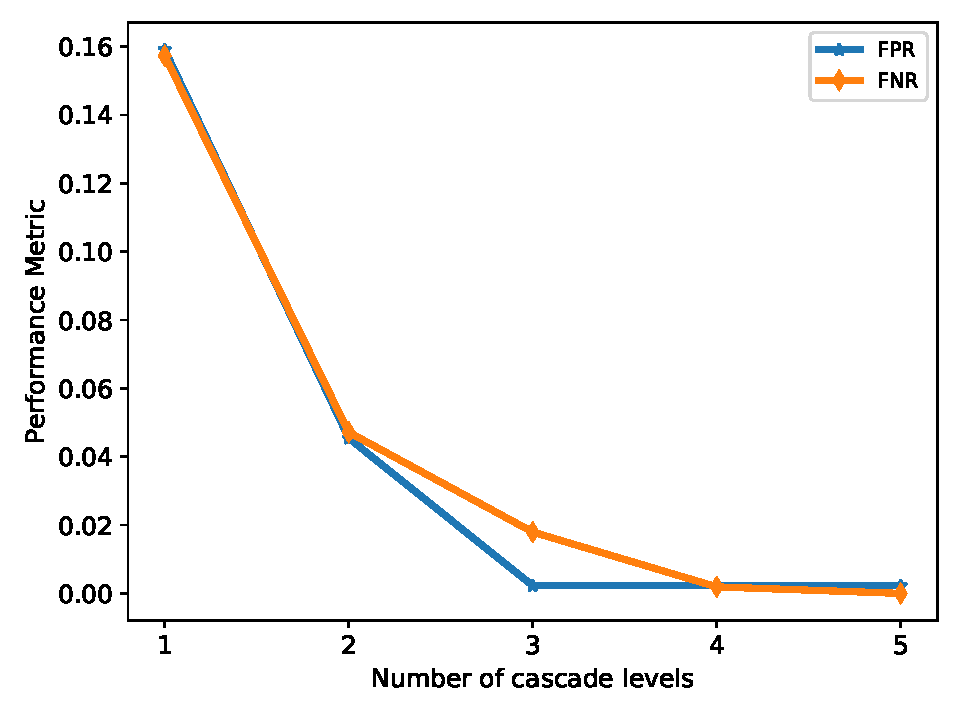
\includegraphics[width=0.32\textwidth]{../My_Code/Results/Adaboost/Adaboost_Performance_5_10_test.pdf}}
    \subcaptionbox{(c)}{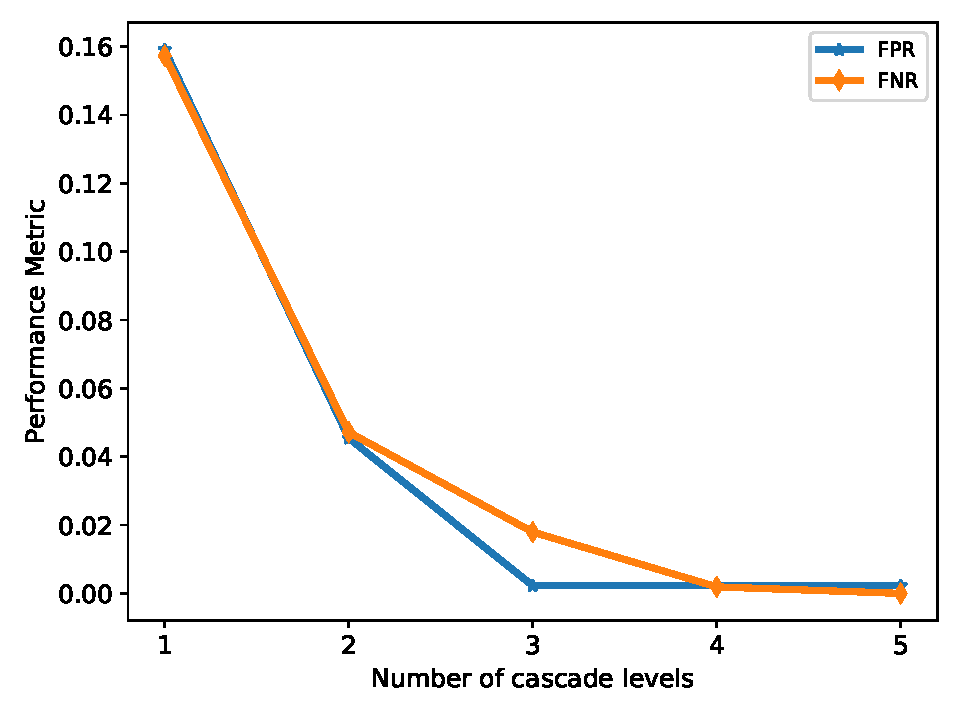
\includegraphics[width=0.32\textwidth]{../My_Code/Results/Adaboost/Adaboost_Performance_20_10_test.pdf}}
    \caption{Propagation of False Positive Rate (FPR) and False Negative Rate (FNR) at each cascading level for different number of iterations. The number of maximum cascading layers is fixed to 10. The number of iterations (N) per cascade level is set to 1 in (a), 5 in (b) and 20 in (c). The FPR reduces within tolerance limit of $10^{-6}$ for FPR in the test set for all three scenarios. It seems when N=1 in (a), the tolerance is not reached within a limit of 10 cascade levels. But for N=5 in (b) or N=20 in (c), the tolerance is reached well within 5 cascade levels. After N=5, there is not much gain in increasing N.}
    \label{fig:adaboost_2}
\end{figure}
\subsection{Comments}
It seems instead of adding successive cascading levels with low number of iterations per cascade levels, it is beneficial to increase number of iterations per cascade level. In helps to find the best weak classifier per cascade level and the corresponding feature vector and threshold. It is evident from the results of both training and test set from FIg. \ref{fig:adaboost_1} and Fig. \ref{fig:adaboost_2}.

\newpage
\section{References}
\begin{itemize}
\item[1.] FacePix Database. URL https://cubic.asu.edu/content/facepix-database.
\item[2.] The AdaBoost Algorithm for Designing Boosted Classifiers, . URL:https://engineering.purdue.edu/kak/Tutorials/AdaBoost.pdf.
\item[3.] Yu, H., \& Yang, J. (2001). A direct LDA algorithm for high-dimensional data—with application to face recognition. Pattern recognition, 34(10), 2067-2070.
\item[4.] Viola, P., \& Jones, M. (2001, December). Rapid object detection using a boosted cascade of simple features. In Proceedings of the 2001 IEEE computer society conference on computer vision and pattern recognition. CVPR 2001 (Vol. 1, pp. I-I). Ieee.
\end{itemize}

\section{Appendix}
\subsection{Source Code - PCA}
\begin{python}
import numpy as np
from scipy import signal
import matplotlib.pyplot as plt
from scipy import linalg
import scipy.io
import cv2,os
import heapq
from collections import Counter

def read_data(data_dir,num_classes,image_per_class):
	labels = list()
	for ix in range(1,num_classes+1):
		for jx in range(1,image_per_class+1):
			class_id = str(ix) if ix >= 10 else '0'+str(ix)
			image_id = str(jx) if jx >= 10 else '0'+str(jx)
			image = cv2.imread(data_dir+'/'+class_id+'_'+image_id+'.png')
			image = cv2.resize(image,(32,32),interpolation = cv2.INTER_AREA)
			if len(image.shape)>2:
				image = cv2.cvtColor(image,cv2.COLOR_BGR2GRAY)
			if ix==1 and jx==1:
				image_shape = image.shape
			image = np.reshape(image.flatten(),[-1,1])
			if ix==1 and jx==1:
				image_set = image
			else:
				image_set = np.concatenate((image_set,image),axis=1)
			labels.append(ix)
	labels = np.array(labels).squeeze()
	return image_set,labels,image_shape
def center_data(data,save_dir):
	mean_data = np.mean(data,axis=1)
	with open(save_dir+'/image_mean.npy', 'wb') as f:
		np.save(f,mean_data)
	data = data - np.reshape(mean_data,[-1,1])
	return data
def normalize_data(data):
	data_norm = np.linalg.norm(data,axis=0)
	data_norm = np.reshape(data_norm,[1,-1])
	data_norm = np.tile(data_norm,(data.shape[0],1))
	data = np.divide(data,data_norm)
	return data
def covariance_matrix(data_set,save_dir,mode='calc'):
	if mode.upper() == "CALC":
		C = np.matmul(data_set,data_set.T)
		C_compressed = np.matmul(data_set.T,data_set)
		with open(save_dir+'/train_data_covariance_matrix.npy', 'wb') as f:
			np.save(f,C)
			np.save(f,C_compressed)
	elif mode.upper() == "LOAD":
		with open(save_dir+'/train_data_covariance_matrix.npy', 'rb') as f:
			C = np.load(f)
			C_compressed = np.load(f)
	return C, C_compressed
def plot_covariance_matrix(C_matrix,save_dir,save_path):
	fig = plt.figure()
	plt.matshow(C_matrix)
	plt.colorbar()
	plt.title('Covariance Matrix')
	plt.savefig(save_dir+'/'+save_path)
def plot_eigenvectors(eigs,K,save_dir):
	plt.figure()
	plt.plot(eigs[:,:K])
	plt.legend(['E'+str(i) for i in range(1,K+1)])
	plt.savefig(save_dir+'/eigenvectors_K_'+str(K)+'.png')
def plot_eigen_faces(eigs,save_dir,image_shape,num_faces):
	count = 0
	num_rows = int(np.sqrt(num_faces))
	num_cols = int(num_faces/float(num_rows))
	eig_f = np.zeros((image_shape[0]*num_rows,image_shape[1]*num_cols))
	for i in range(0,num_faces):
		row = int(np.floor((i)/num_cols))*image_shape[0]
		col = count*image_shape[1]
		eig_f[row:row+image_shape[0],col:col+image_shape[1]] = np.reshape(eigs[:,i],list(image_shape))
		count += 1
		if count >= num_cols:
			count = 0
	plt.figure()
	plt.imshow(eig_f)
	plt.savefig(save_dir+'/Eigen_Faces.png')
def calculate_K_large_eigenvectors(data,C_matrix_compressed,K,image_shape,save_dir,mode='calc'):
	if mode.upper() == "CALC":
		[w,u] = np.linalg.eig(C_matrix_compressed)#w=eigenvalues, v=eigenvectors; the column v[:,i] is the eigenvector corresponding to the eigenvalue w[i].
		v = np.matmul(data,u)
		v = np.real(v)
		#normalize eigenvectors
		v = v/np.linalg.norm(v,axis=0)
		with open(save_dir+'/eigs.npy', 'wb') as f:
			np.save(f, w)
			np.save(f, v)
		w = np.abs(w)
		ws = heapq.nlargest(K, w)
		ind = [list(w).index(i) for i in ws]
		Q = v[:,ind]
		with open(save_dir+'/eigenvectors.npy', 'wb') as f:
			np.save(f,Q)
	elif mode.upper() == "LOAD":
		with open(save_dir+'/eigs.npy', 'rb') as f:
			w = np.load(f)
			v = np.load(f)
		with open(save_dir+'/eigenvectors.npy', 'rb') as f:
			Q = np.load(f)
	#plot_eigenvectors(Q,K,save_dir)
	if K==49:
		plot_eigen_faces(np.abs(Q),save_dir,image_shape,K)
	return Q[:,:K],v[:,:K],w[:K]
def get_low_dimensional_projections(v,Q,data,save_dir):
	ak = list()
	bk = list()
	ck = list()
	for i in range(0,data.shape[1]):
		ak.append(np.dot(data[:,i],Q[:,0]))
		bk.append(np.dot(data[:,i],Q[:,1]))
		ck.append(np.dot(data[:,i],Q[:,2]))

	ak,bk,ck = np.array(ak),np.array(bk),np.array(ck)
	fig = plt.figure()
	ax = fig.add_subplot(projection='3d')
	ax.scatter(ak,bk,ck)
	ax.set_xlabel('eig_0')
	ax.set_ylabel('eig_1')
	ax.set_zlabel('eig_2')
	plt.savefig(save_dir+'/projectioins_along_first_three_eig.png')
	return ak,bk,ck
def get_gt_coeffs(data,Q,K,image_shape,save_dir):
	coeff = np.matmul(data.T,Q)
	with open(save_dir+'/coefficients.npy', 'wb') as f:
		np.save(f,coeff)
	return coeff
def get_prediction(data,Q,K,image_shape,save_dir):
	with open(save_dir+'/image_mean.npy', 'rb') as f:
		image_mean = np.reshape(np.load(f),[-1,1])

	with open(save_dir+'/coefficients.npy', 'rb') as f:
		coeff_gt = np.load(f)
	data = data - image_mean
	data = normalize_data(data)
	coeff_pred = np.matmul(data.T,Q)
	distance = np.zeros((data.shape[1],coeff_gt.shape[0]))
	for ix in range(0,data.shape[1]):
		distance[ix,:] = np.sqrt(np.sum(np.square(coeff_gt-coeff_pred[ix,:]),axis=1)).T
	return distance
def calculate_accuracy(y_true,distance,image_per_class,num_classes,method="L2",params=None):
	if method.upper() == "L2":
		match_ind = np.argmin(distance,axis=1)+1#+1 is for indices start from 1
		y_pred = y_true[match_ind]
		y_pred = y_pred.astype(int).squeeze()

	elif method.upper() == "KNN":
		num_neighbours = params[0]
		y_pred = list()
		for im in range(0,distance.shape[0]):
			dist = distance[im,:]
			class_hits = np.zeros((num_classes))
			class_dist = np.zeros((num_classes))
			for ix in range(0,num_neighbours):
				min_idx = np.argmin(dist)
				min_label = y_true[min_idx]-1
				class_hits[min_label] += 1
				class_dist[min_label] += dist[min_idx]
				dist[min_idx] = float('inf')
			max_hits = np.max(class_hits)
			class_avg_dist = class_dist/max_hits
			class_avg_dist = np.where(class_avg_dist==0,np.inf,class_avg_dist)
			class_id = np.argmin(class_avg_dist)+1
			y_pred.append(class_id)
		y_pred = np.array(y_pred).astype(int).squeeze()

	match = np.where(y_true==y_pred,1,0)
	correct_labels = np.sum(match)
	accuracy = correct_labels/y_true.shape[0]*100
	return accuracy
def main():
	train_dir = '../FaceRecognition/train'
	test_dir = '../FaceRecognition/test'
	save_dir = './Results/PCA'
	if not os.path.exists(save_dir):
		os.makedirs(save_dir)

	num_classes = 30
	train_image_per_class = 21
	test_image_per_class = 21
	classifier = "KNN"#options = KNN,L2
	params = [1]
	Kmax = 25

	X_train,Y_train,image_shape = read_data(train_dir,num_classes,train_image_per_class)
	X_test,Y_test,_ = read_data(test_dir,num_classes,test_image_per_class)
	X_train = center_data(X_train,save_dir)
	X_train = normalize_data(X_train)
	print('Train data = ',X_train.shape)
	print('Test data = ',X_test.shape)
	C_matrix,C_matrix_compressed = covariance_matrix(X_train,save_dir,mode='calc')
	print('C_matrix_train = ',C_matrix.shape)
	print('C_matrix_compressed_train = ',C_matrix_compressed.shape)
	plot_covariance_matrix(C_matrix,save_dir,'train_data_covariance_matrix.png')
	Accuracies = list()
	for K in range(1,Kmax+1,1):
		[Q,v,w] = calculate_K_large_eigenvectors(X_train,C_matrix_compressed,K,image_shape,save_dir,mode='calc')
		#[ak,bk,ck] = get_low_dimensional_projections(v,Q,X_train,save_dir)
		coeff = get_gt_coeffs(X_train,Q,K,image_shape,save_dir)
		distance = get_prediction(X_test,Q,K,image_shape,save_dir)
		accuracy = calculate_accuracy(Y_test,distance,test_image_per_class,num_classes,method=classifier,params=params)
		print("K = ",K,", Accuracy = ",accuracy,'%')
		Accuracies.append(accuracy)
		with open(save_dir+'/PCA_Accuracies.npy', 'wb') as f:
			np.save(f,Accuracies)
main()

\end{python}
\subsection{Source Code - LDA}
\begin{python}
import numpy as np
from scipy import signal
import matplotlib.pyplot as plt
from scipy import linalg
import scipy.io
import cv2,os
import heapq
from collections import Counter
import gzip, pickle, pickletools

def read_data(data_dir,num_classes,image_per_class):
	labels = list()
	for ix in range(1,num_classes+1):
		for jx in range(1,image_per_class+1):
			class_id = str(ix) if ix >= 10 else '0'+str(ix)
			image_id = str(jx) if jx >= 10 else '0'+str(jx)
			image = cv2.imread(data_dir+'/'+class_id+'_'+image_id+'.png')
			image = cv2.resize(image,(32,32),interpolation = cv2.INTER_AREA)
			if len(image.shape)>2:
				image = cv2.cvtColor(image,cv2.COLOR_BGR2GRAY)
			if ix==1 and jx==1:
				image_shape = image.shape
			image = np.reshape(image.flatten(),[-1,1])
			if ix==1 and jx==1:
				image_set = image
			else:
				image_set = np.concatenate((image_set,image),axis=1)
			labels.append(ix)
	labels = np.array(labels).squeeze()
	return image_set,labels,image_shape
def center_data(data):
	mean_data = np.mean(data,axis=1)
	data = data - np.reshape(mean_data,[-1,1])
	return data
def normalize_data(data):
	data_norm = np.linalg.norm(data,axis=0)
	data_norm = np.reshape(data_norm,[1,-1])
	data_norm = np.tile(data_norm,(data.shape[0],1))
	data = np.divide(data,data_norm)
	return data
def lda_mean_calculation(data,num_classes,image_per_class,save_dir,lda_mode):
	for ix in range(0,num_classes):
		class_data = data[:,ix*image_per_class:(ix+1)*image_per_class]
		mean_class_data = np.mean(class_data,axis=1).reshape([-1,1])
		if ix == 0:
			within_class_mean = mean_class_data
		else:
			within_class_mean = np.concatenate((within_class_mean,mean_class_data),axis=1)
	global_mean = np.mean(data,axis=1).reshape([-1,1])
	with open(save_dir+'/lda_means_'+lda_mode+'.pkl','wb') as f:
		pickle.dump(within_class_mean,f)
		pickle.dump(global_mean,f)
	return within_class_mean,global_mean
def calculate_scatter_matrices(data,within_class_mean,global_mean,num_classes,image_per_class,save_dir,lda_mode,mode='calc'):
	if mode.upper()=="CALC":
		M = within_class_mean-global_mean
		SB = np.matmul(M,M.T)/within_class_mean.shape[1]
		SW = np.zeros(SB.shape)
		for ix in range(0,num_classes):
			class_data = data[:,ix*image_per_class:(ix+1)*image_per_class]
			M = class_data - np.reshape(within_class_mean[:,ix],[-1,1])
			SW += np.matmul(M,M.T)/float(image_per_class)
		SW = SW/float(num_classes)
		combined_scatter_matrix = np.matmul(np.linalg.pinv(SW),SB)
		with open(save_dir+'/scatter_matrices_'+lda_mode+'.pkl','wb') as f:
			pickle.dump(SW,f)
			pickle.dump(SB,f)
			pickle.dump(combined_scatter_matrix,f)
	elif mode.upper() == "LOAD":
		print("Loading Scatter Matrices")
		with open(save_dir+'/scatter_matrices_'+lda_mode+'.pkl', 'rb') as f:
			SB = pickle.load(f)
			SW = pickle.load(f)
			combined_scatter_matrix = pickle.load(f)
	else:
		print("Please specify a correct mode of operation, either 'calc' or 'load'")
	return SB,SW,combined_scatter_matrix
def plot_eigenvectors(eigs,K,save_dir,lda_mode):
	plt.figure()
	plt.plot(eigs[:,:K])
	plt.legend(['E'+str(i) for i in range(1,K+1)])
	plt.savefig(save_dir+'/eigenvectors_K_'+str(K)+'_'+lda_mode+'.png')
def plot_covariance_matrix(C_matrix,save_dir,save_path,title):
	fig = plt.figure()
	C_matrix = C_matrix/np.max(C_matrix)
	plt.matshow(C_matrix)
	plt.colorbar()
	plt.title(title)
	plt.savefig(save_dir+'/'+save_path)
def calculate_K_large_eigenvectors(SB,SW,combined_scatter_matrix,K,save_dir,lda_mode,lda_mode_params,mode='calc'):
	if mode.upper() == "CALC":
		if lda_mode.upper()=="ORIGINAL":
			[w,v] = np.linalg.eig(combined_scatter_matrix)
			v = np.abs(v)
			v = v/np.linalg.norm(v,axis=0)
			with open(save_dir+'/eigs_'+lda_mode+'.pkl', 'wb') as f:
				pickle.dump(w,f)
				pickle.dump(v,f)
			w = np.abs(w)
			ws = heapq.nlargest(K, w)
			ind = [list(w).index(i) for i in ws]
			Q = v[:,ind]
			with open(save_dir+'/eigenvectors_'+lda_mode+'.pkl', 'wb') as f:
				pickle.dump(Q,f)
			del v
		elif lda_mode.upper()=="YU_YANG":
			KY = lda_mode_params[0]
			[w,v] = np.linalg.eig(SB)
			v = np.real(v)
			v = v/np.linalg.norm(v,axis=0)
			w = np.abs(w)
			ws = heapq.nlargest(KY, w)
			ind = [list(w).index(i) for i in ws]
			Y = v[:,ind]
			DB = w[ind]
			Z = np.matmul(Y,np.diag(1/np.sqrt(DB)))
			G = np.matmul(Z.T,np.matmul(SW,Z))
			[wg,vg] = np.linalg.eig(G)
			vg = np.real(vg)
			vg = vg/np.linalg.norm(vg,axis=0)
			wg = np.abs(wg)
			wgs = heapq.nsmallest(K, wg)
			indg = [list(wg).index(i) for i in wgs]
			U = vg[:,indg]
			Q = np.matmul(U.T,Z.T).T
			with open(save_dir+'/eigenvectors_'+lda_mode+'.pkl', 'wb') as f:
				pickle.dump(Q,f)
	elif mode.upper() == "LOAD":
		#print("Loading Eigenvectors")
		with open(save_dir+'/eigenvectors_'+lda_mode+'.pkl', 'rb') as f:
			Q = pickle.load(f)
	#plot_eigenvectors(Q,K,save_dir)
	return Q[:,:K]
def get_gt_coeffs(data,global_mean,Q,K,image_shape,save_dir,lda_mode):
	data = data - global_mean
	coeff = np.matmul(data.T,Q)
	with open(save_dir+'/coefficients_'+lda_mode+'.pkl', 'wb') as f:
		pickle.dump(coeff,f)
	return coeff
def get_prediction(data,Q,K,image_shape,save_dir,lda_mode):
	with open(save_dir+'/lda_means_'+lda_mode+'.pkl', 'rb') as f:
		within_class_mean = pickle.load(f)
		image_mean = np.reshape(pickle.load(f),[-1,1])#Loading the global mean which is the last pickle inside the pkl file

	with open(save_dir+'/coefficients_'+lda_mode+'.pkl', 'rb') as f:
		coeff_gt = pickle.load(f)
	data = data - image_mean
	coeff_pred = np.matmul(data.T,Q)
	distance = np.zeros((data.shape[1],coeff_gt.shape[0]))
	for ix in range(0,data.shape[1]):
		distance[ix,:] = np.sqrt(np.sum(np.square(coeff_gt-coeff_pred[ix,:]),axis=1)).T
	return distance
def calculate_accuracy(y_true,distance,image_per_class,num_classes,method="L2",params=None):
	if method.upper() == "L2":
		match_ind = np.argmin(distance,axis=1)+1#+1 is for indices start from 1
		y_pred = y_true[match_ind]
		y_pred = y_pred.astype(int).squeeze()
	elif method.upper() == "KNN":
		num_neighbours = params[0]
		y_pred = list()
		for im in range(0,distance.shape[0]):
			dist = distance[im,:]
			class_hits = np.zeros((num_classes))
			class_dist = np.zeros((num_classes))
			for ix in range(0,num_neighbours):
				min_idx = np.argmin(dist)
				min_label = y_true[min_idx]-1
				class_hits[min_label] += 1
				class_dist[min_label] += dist[min_idx]
				dist[min_idx] = float('inf')
			max_hits = np.max(class_hits)
			class_avg_dist = class_dist/max_hits
			class_avg_dist = np.where(class_avg_dist==0,np.inf,class_avg_dist)
			class_id = np.argmin(class_avg_dist)+1
			y_pred.append(class_id)
		y_pred = np.array(y_pred).astype(int).squeeze()

	match = np.where(y_true==y_pred,1,0)
	correct_labels = np.sum(match)
	accuracy = correct_labels/y_true.shape[0]*100
	return accuracy
def main():
	train_dir = '../FaceRecognition/train'
	test_dir = '../FaceRecognition/test'
	save_dir = './Results/LDA'
	if not os.path.exists(save_dir):
		os.makedirs(save_dir)

	num_classes = 30
	train_image_per_class = 21
	test_image_per_class = 21
	classifier = "KNN"#options = KNN,L2
	params = [1]
	Kmax = 25
	lda_mode = "yu_yang"#options = "yu_yang","original"
	lda_mode_params = [11]#eigenvectors to keep in Yu-Yang's algorithm

	X_train,Y_train,image_shape = read_data(train_dir,num_classes,train_image_per_class)
	X_train = normalize_data(X_train)
	X_test,Y_test,_ = read_data(test_dir,num_classes,test_image_per_class)
	X_test = normalize_data(X_test)
	print('Train data = ',X_train.shape)
	print('Test data = ',X_test.shape)
	within_class_mean,global_mean = lda_mean_calculation(X_train,num_classes,train_image_per_class,save_dir,lda_mode)
	SB,SW,combined_scatter_matrix = calculate_scatter_matrices(X_train,within_class_mean,global_mean,num_classes,train_image_per_class,save_dir,lda_mode,mode='calc')
	print('SB = ',SB.shape)
	print('SW = ',SW.shape)
	plot_covariance_matrix(SB,save_dir,'train_data_SB_'+lda_mode+'.png','SB')
	plot_covariance_matrix(SW,save_dir,'train_data_SW_'+lda_mode+'.png','SW')
	plot_covariance_matrix(combined_scatter_matrix,save_dir,'train_data_combined_scatter_matrix_'+lda_mode+'.png','$SW^{-1}SB$')
	Accuracies = list()
	for K in range(1,Kmax+1,1):
		Q = calculate_K_large_eigenvectors(SB,SW,combined_scatter_matrix,K,save_dir,lda_mode,lda_mode_params,mode='calc')
		#[ak,bk,ck] = get_low_dimensional_projections(v,Q,X_train,save_dir)
		coeff = get_gt_coeffs(X_train,global_mean,Q,K,image_shape,save_dir,lda_mode)
		distance = get_prediction(X_test,Q,K,image_shape,save_dir,lda_mode)
		accuracy = calculate_accuracy(Y_test,distance,test_image_per_class,num_classes,method=classifier,params=params)
		print("lda_mode = "+lda_mode+", K = ",K,", Accuracy = ",accuracy,'%')
		Accuracies.append(accuracy)
		with open(save_dir+'/LDA_Accuracies_'+lda_mode+'.npy', 'wb') as f:
			np.save(f,Accuracies)

main()

\end{python}
\subsection{Source Code - Autoencoder}
\begin{python}
import os

import numpy as np
import torch
from torch import nn, optim
from PIL import Image
from torch.autograd import Variable
from torch.utils.data import Dataset, DataLoader
from torchvision import transforms


class DataBuilder(Dataset):
	def __init__(self, path):
		self.path = path
		self.image_list = [f for f in os.listdir(path) if f.endswith('.png')]
		self.label_list = [int(f.split('_')[0]) for f in self.image_list]
		self.len = len(self.image_list)
		self.aug = transforms.Compose([
			transforms.Resize((64, 64)),
			transforms.ToTensor(),
		])

	def __getitem__(self, index):
		fn = os.path.join(self.path, self.image_list[index])
		x = Image.open(fn).convert('RGB')
		x = self.aug(x)
		return {'x': x, 'y': self.label_list[index]}

	def __len__(self):
		return self.len
class Autoencoder(nn.Module):

	def __init__(self, encoded_space_dim):
		super().__init__()
		self.encoded_space_dim = encoded_space_dim
		### Convolutional section
		self.encoder_cnn = nn.Sequential(
			nn.Conv2d(3, 8, 3, stride=2, padding=1),
			nn.LeakyReLU(True),
			nn.Conv2d(8, 16, 3, stride=2, padding=1),
			nn.LeakyReLU(True),
			nn.Conv2d(16, 32, 3, stride=2, padding=1),
			nn.LeakyReLU(True),
			nn.Conv2d(32, 64, 3, stride=2, padding=1),
			nn.LeakyReLU(True)
		)
		### Flatten layer
		self.flatten = nn.Flatten(start_dim=1)
		### Linear section
		self.encoder_lin = nn.Sequential(
			nn.Linear(4 * 4 * 64, 128),
			nn.LeakyReLU(True),
			nn.Linear(128, encoded_space_dim * 2)
		)
		self.decoder_lin = nn.Sequential(
			nn.Linear(encoded_space_dim, 128),
			nn.LeakyReLU(True),
			nn.Linear(128, 4 * 4 * 64),
			nn.LeakyReLU(True)
		)
		self.unflatten = nn.Unflatten(dim=1, unflattened_size=(64, 4, 4))
		self.decoder_conv = nn.Sequential(
			nn.ConvTranspose2d(64, 32, 3, stride=2,padding=1, output_padding=1),
			nn.BatchNorm2d(32),
			nn.LeakyReLU(True),
			nn.ConvTranspose2d(32, 16, 3, stride=2,padding=1, output_padding=1),
			nn.BatchNorm2d(16),
			nn.LeakyReLU(True),
			nn.ConvTranspose2d(16, 8, 3, stride=2,padding=1, output_padding=1),
			nn.BatchNorm2d(8),
			nn.LeakyReLU(True),
			nn.ConvTranspose2d(8, 3, 3, stride=2,padding=1, output_padding=1)
		)

	def encode(self, x):
		x = self.encoder_cnn(x)
		x = self.flatten(x)
		x = self.encoder_lin(x)
		mu, logvar = x[:, :self.encoded_space_dim], x[:, self.encoded_space_dim:]
		return mu, logvar

	def decode(self, z):
		x = self.decoder_lin(z)
		x = self.unflatten(x)
		x = self.decoder_conv(x)
		x = torch.sigmoid(x)
		return x

	@staticmethod
	def reparameterize(mu, logvar):
		std = logvar.mul(0.5).exp_()
		eps = Variable(std.data.new(std.size()).normal_())
		return eps.mul(std).add_(mu)
class VaeLoss(nn.Module):
	def __init__(self):
		super(VaeLoss, self).__init__()
		self.mse_loss = nn.MSELoss(reduction="sum")

	def forward(self, xhat, x, mu, logvar):
		loss_MSE = self.mse_loss(xhat, x)
		loss_KLD = -0.5 * torch.sum(1 + logvar - mu.pow(2) - logvar.exp())
		return loss_MSE + loss_KLD
def train(epoch,epochs,p):
	model.train()
	train_loss = 0

	for batch_idx, data in enumerate(trainloader):
		optimizer.zero_grad()
		mu, logvar = model.encode(data['x'])
		z = model.reparameterize(mu, logvar)
		xhat = model.decode(z)
		loss = vae_loss(xhat, data['x'], mu, logvar)
		loss.backward()
		train_loss += loss.item()
		optimizer.step()

	print('====> P: {} Epoch: {}/{} Average loss: {:.4f}'.format(p,epoch,epochs, train_loss / len(trainloader.dataset)))
def calculate_accuracy(y_true,distance,image_per_class,num_classes,method="L2",params=None):
	if method.upper() == "L2":
		match_ind = np.argmin(distance,axis=1)+1#+1 is for indices start from 1
		y_pred = y_true[match_ind]
		y_pred = y_pred.astype(int).squeeze()

	elif method.upper() == "KNN":
		num_neighbours = params[0]
		y_pred = list()
		for im in range(0,distance.shape[0]):
			dist = distance[im,:]
			class_hits = np.zeros((num_classes))
			class_dist = np.zeros((num_classes))
			for ix in range(0,num_neighbours):
				min_idx = np.argmin(dist)
				min_label = y_true[min_idx]-1
				class_hits[min_label] += 1
				class_dist[min_label] += dist[min_idx]
				dist[min_idx] = float('inf')
			max_hits = np.max(class_hits)
			class_avg_dist = class_dist/max_hits
			class_avg_dist = np.where(class_avg_dist==0,np.inf,class_avg_dist)
			class_id = np.argmin(class_avg_dist)+1
			y_pred.append(class_id)
		y_pred = np.array(y_pred).astype(int).squeeze()
	match = np.where(y_true==y_pred,1,0)
	correct_labels = np.sum(match)
	accuracy = correct_labels/y_true.shape[0]*100
	return accuracy
##################################
# Change these
#device = torch.device('cuda' if torch.cuda.is_available() else 'cpu')
device = 'cpu'
print(device)
training = False
pretrained_weights = False


TRAIN_DATA_PATH =  '../FaceRecognition/train'
EVAL_DATA_PATH = '../FaceRecognition/test'
OUT_PATH = './Results/autoencoder_outputs'
if pretrained_weights:
	WEIGHT_DIR = './autoencoder_weights'
	P = [3,8,16]
else:
	WEIGHT_DIR = './Results/autoencoder_outputs'
	P = np.arange(1,26,1)
num_classes = 30
train_image_per_class = 21
test_image_per_class = 21
classifier = "KNN"#options = KNN,L2
params = [1]#KNN neighbour
if not os.path.exists(OUT_PATH):
	os.makedirs(OUT_PATH)
##################################
Accuracies = list()
for p in P:
	LOAD_PATH = WEIGHT_DIR+'/model_'+str(p)+'.pt'
	model = Autoencoder(p)

	if training:
		epochs = 100
		log_interval = 1
		trainloader = DataLoader(
			dataset=DataBuilder(TRAIN_DATA_PATH),
			batch_size=12,
			shuffle=True,
		)
		optimizer = optim.Adam(model.parameters(), lr=1e-3)
		vae_loss = VaeLoss()
		for epoch in range(1, epochs + 1):
			train(epoch,epochs,p)
		torch.save(model.state_dict(), os.path.join(OUT_PATH, f'model_{p}.pt'))
	else:
		trainloader = DataLoader(
			dataset=DataBuilder(TRAIN_DATA_PATH),
			batch_size=1,
		)

		model.load_state_dict(torch.load(LOAD_PATH))
		model.eval()
		model.to(device)

		X_train = []
		Y_train = []
		for batch_idx, data in enumerate(trainloader):
			mu, logvar = model.encode(data['x'])
			z = mu.detach().cpu().numpy().flatten()
			X_train.append(z)
			Y_train.append(data['y'].item())
		X_train = np.stack(X_train)
		Y_train = np.array(Y_train)

		testloader = DataLoader(
			dataset=DataBuilder(EVAL_DATA_PATH),
			batch_size=1,
		)
		X_test, Y_test = [], []
		for batch_idx, data in enumerate(testloader):
			mu, logvar = model.encode(data['x'])
			z = mu.detach().cpu().numpy().flatten()
			X_test.append(z)
			Y_test.append(data['y'].item())
		X_test = np.stack(X_test)
		Y_test = np.array(Y_test)

		distance = np.zeros((X_test.shape[0],X_train.shape[0]))

		for ix in range(0,X_test.shape[0]):
			distance[ix,:] = np.sqrt(np.sum(np.square(X_train-X_test[ix,:]),axis=1)).T
		accuracy = calculate_accuracy(Y_test,distance,test_image_per_class,num_classes,method=classifier,params=params)
		print("P = ",p,", Accuracy = ",accuracy,'%')
		Accuracies.append(accuracy)
	if pretrained_weights:
		fname = OUT_PATH+'/Autoencoder_Accuracies_pretrained.npy'
	else:
		fname = OUT_PATH+'/Autoencoder_Accuracies_custom_trained.npy'
	with open(fname, 'wb') as f:
		np.save(f,Accuracies)

\end{python}
\subsection{Source Code - Cascaded AdaBoost}
\begin{python}
import numpy as np
import os
import cv2
import matplotlib.pyplot as plt
import gzip, pickle, pickletools

def calculate_features(img):
	if len(img.shape)>2:
		img = cv2.cvtColor(img,cv2.COLOR_BGR2GRAY)
	window_widths = np.arange(2,img.shape[1],2)
	window_heights = np.arange(2,img.shape[0],2)
	features = list()
	for N in window_widths:
		img_padded = np.pad(img,((0,0),(int(N/2),int(N/2))),mode='constant')
		for ix in range(0,img.shape[0]):
			for jx in range(int(N/2),img_padded.shape[1]-int(N/2)+1):
				neg_sums = np.sum(img_padded[ix,jx-int(N/2):jx+1].flatten()).astype(np.int32)
				pos_sums = np.sum(img_padded[ix,jx+1:jx+int(N/2)+1].flatten()).astype(np.int32)
				features.append(pos_sums-neg_sums)

	for N in window_heights:
		img_padded = np.pad(img,((int(N/2),int(N/2)),(0,0)),mode='constant')
		for ix in range(int(N/2),img_padded.shape[0]-int(N/2)+1):
			for jx in range(0,img.shape[1]):
				neg_sums = np.sum(img_padded[ix-int(N/2):ix+1,jx].flatten()).astype(np.int32)
				pos_sums = np.sum(img_padded[ix+1:ix+int(N/2)+1,jx].flatten()).astype(np.int32)
				features.append(pos_sums-neg_sums)

	features = np.array(features)
	return features
def extract_features(classes,data_dir,Result_dir,name):
	print("Constructing feature matrices for the dataset")
	for C in classes:
		save_path = Result_dir+'/'+name+'_'+C+'.npy'
		if not os.path.exists(save_path):
			features = list()
			path_dir = data_dir+'/'+C
			for F in os.listdir(path_dir):
				print('name '+C+' Images = ',len(features),end="\r")
				image = cv2.imread(path_dir+'/'+F)
				features.append(calculate_features(image))
			features = np.array(features)
			features = np.reshape(features,[len(features),-1])
			np.save(save_path,features)
			print("\n")
		else:
			print('Found feature matrices alredy in ',save_path,end=' ')
			if C.upper()=="POSITIVE":
				data_pos_features = np.load(save_path)
				print(' ===> ',data_pos_features.shape)
			elif C.upper()=="NEGATIVE":
				data_neg_features = np.load(save_path)
				print(' ===> ',data_neg_features.shape)
	return data_pos_features,data_neg_features
def create_labels(pos_features,neg_features):
	combined_features = np.concatenate((pos_features,neg_features),axis=0)
	combined_labels = np.concatenate((np.ones((pos_features.shape[0],1)), np.zeros((neg_features.shape[0],1))), axis=0).astype(np.uint8)
	return combined_features,combined_labels.squeeze()
def create_weak_classifier(features,labels,weights):
	classifier_error = np.float64('inf')
	#iterate over each feature across images
	for F in range(0,features.shape[1]):
		feature_vector = features[:,F]
		indx = np.argsort(feature_vector)
		feature_vector_sorted,labels_sorted,weights_sorted = feature_vector[indx],labels[indx],weights[indx]
		positive_weights = np.zeros((features.shape[0],1))
		negative_weights = np.zeros((features.shape[0],1))
		positive_weights[labels_sorted==1,0] = weights_sorted[labels_sorted==1]
		negative_weights[labels_sorted==0,0] = weights_sorted[labels_sorted==0]

		error_pol_1 = np.reshape(np.cumsum(positive_weights) + np.sum(negative_weights) - np.cumsum(negative_weights), [-1,1])
		error_pol_2 = np.reshape(np.cumsum(negative_weights) + np.sum(positive_weights) - np.cumsum(positive_weights), [-1,1])
		error = np.concatenate((error_pol_1,error_pol_2),axis=1)
		min_idx = np.unravel_index(np.argmin(error),error.shape)
		min_err = error[min_idx]

		#weak classifier update
		if min_err < classifier_error:
			classifier_error = min_err
			feature_idx = F
			threshold = feature_vector_sorted[min_idx[0]]
			polarity = 1 if min_idx[1]==0 else 0
			classifications = feature_vector>=threshold if polarity==1 else feature_vector<threshold
			classifier = [feature_idx,threshold,polarity,classifier_error,classifications]
	return classifier
def create_adaboost_cascade(features,labels,iterations_per_cascade,cascade_level):
	weights = np.concatenate((np.repeat(1/np.sum(labels==1),np.sum(labels==1)), np.repeat(1/np.sum(labels==0),np.sum(labels==0))),axis=0)
	best_classifier = None
	best_trust_factor = -np.float64('inf')
	for iter in range (iterations_per_cascade):
		weights = weights/np.sum(weights)#normalize the weights
		class_feature_idx,class_thresh,class_polarity,class_error,class_predicted_labels = create_weak_classifier(features,labels,weights)
		class_predicted_labels = np.where(class_predicted_labels==0,-1,class_predicted_labels)
		epsilon_t = np.matmul(np.reshape(weights,[1,-1]),np.abs(class_predicted_labels-labels).reshape(-1,1)).squeeze()*0.5
		trust_factor = np.log((1-epsilon_t)/epsilon_t) * 0.5
		#update the weights
		weights = weights * np.exp(-trust_factor*labels*class_predicted_labels)

		FPR = np.sum(class_predicted_labels[np.sum(labels==1):]==1)/np.sum(labels==0)
		FNR = 1 - (np.sum(class_predicted_labels[:np.sum(labels==1)]==1)/np.sum(labels==1))

		print('Cascade Level = ',cascade_level+1,' Iteration = ',iter+1,' epsilon_t = ',round(epsilon_t,4),' trust_factor = ',round(trust_factor,4),' #Negatives = ',np.sum(labels==0),' FPR = ',round(FPR*100,4),'% FNR = ',round(FNR*100,4),'%')
		if trust_factor > best_trust_factor:
			best_trust_factor = trust_factor
			best_class_predictions = class_predicted_labels
			best_FPR = FPR
			best_FNR = FNR
			best_weak_classifier = [class_feature_idx,class_thresh,class_polarity,class_error,class_predicted_labels,FPR,FNR,epsilon_t,trust_factor]

	#revise the dataset for the next cascade layer
	#find out all the detections that have been classified as positive
	new_pos_features = features[:np.sum(labels==1),:]
	new_neg_features = features[np.sum(labels==1):,:]
	new_neg_features = new_neg_features[np.where(best_class_predictions[np.sum(labels==1):] == 1),:][0]
	new_features,new_labels = create_labels(new_pos_features,new_neg_features)
	del new_pos_features,new_neg_features
	return new_features,new_labels,best_FPR,best_FNR,best_weak_classifier
def plot_cascade_adaboost_performance(FPRs,FNRs,iterations_per_cascade,num_cascades,save_dir,name,title=None):
	SMALL_SIZE = 10
	MEDIUM_SIZE = 12
	BIGGER_SIZE = 14
	LINE_WIDTH=3
	plt.rc('font', size=SMALL_SIZE)
	plt.rc('axes', titlesize=SMALL_SIZE)     # fontsize of the axes title
	plt.rc('axes', labelsize=MEDIUM_SIZE)    # fontsize of the x and y labels
	plt.rc('xtick', labelsize=MEDIUM_SIZE)    # fontsize of the tick labels
	plt.rc('ytick', labelsize=MEDIUM_SIZE)    # fontsize of the tick labels
	plt.rc('legend', fontsize=SMALL_SIZE)    # legend fontsize
	plt.rc('figure', titlesize=BIGGER_SIZE)  # fontsize of the figure title
	fig = plt.figure()
	plt.plot(FPRs,'-*',label='FPR', linewidth=LINE_WIDTH)
	plt.plot(FNRs,'-d',label='FNR', linewidth=LINE_WIDTH)
	plt.legend()
	plt.xlabel('Number of cascade levels')
	plt.ylabel('Performance Metric')
	plt.xticks(np.arange(0,len(FPRs),1), [str(ix) for ix in range(1,len(FPRs)+1,1)])
	plt.title(title)
	plt.tight_layout()
	plt.savefig(save_dir+'/Adaboost_Performance_'+str(iterations_per_cascade)+'_'+str(num_cascades)+'_'+name+'.pdf')
	plt.savefig(save_dir+'/Adaboost_Performance_'+str(iterations_per_cascade)+'_'+str(num_cascades)+'_'+name+'.png',dpi=600)
def inference(Best_Classifier_Per_Cascade_Level,features,labels):
	Final_classification_labels = np.ones((features.shape[0],1))
	global_class_idx = np.arange(0,features.shape[0],1).reshape(-1,1)
	actual_positive_samples = np.sum(labels==1)
	actual_negative_samples = np.sum(labels==0)
	FPRs = list()
	FNRs = list()
	for ix in range(0,len(Best_Classifier_Per_Cascade_Level)):
		feature_ID = Best_Classifier_Per_Cascade_Level[str(ix+1)][0]
		threshold = Best_Classifier_Per_Cascade_Level[str(ix+1)][1]
		polarity = Best_Classifier_Per_Cascade_Level[str(ix+1)][2]
		trust_factor = Best_Classifier_Per_Cascade_Level[str(ix+1)][-1]

		feature_vector = features[:,feature_ID].reshape([-1,1])
		classifications = feature_vector>=threshold if polarity==1 else feature_vector<threshold
		classifications = np.where(classifications==0,-1,classifications)
		total_classifications = trust_factor*classifications
		final_classifications = total_classifications >= trust_factor

		if np.sum(labels==0) == 0:
			FPR = 0
		else:
			FPR = np.sum(final_classifications[np.sum(labels==1):]==1)/np.sum(labels==0)
		if np.sum(labels==1) == 0:
			FNR=0
		else:
			FNR = 1 - (np.sum(final_classifications[:np.sum(labels==1)]==1)/np.sum(labels==1))


		features = features[np.where(final_classifications == 1),:][0]
		labels = labels[np.where(final_classifications == 1)[0]]
		global_negative_class_idx = global_class_idx[np.where(final_classifications == 0),:][0]
		Final_classification_labels[global_negative_class_idx,0] = -1
		global_class_idx = global_class_idx[np.where(final_classifications==1),:][0]
		if ix==0:
			Test_Predictions = Final_classification_labels
			FPRs.append(FPR)
			FNRs.append(FNR)
		else:
			Test_Predictions = np.concatenate((Test_Predictions,Final_classification_labels),axis=1)
			FPRs.append(FPRs[-1]*FPR)
			FNRs.append(FNRs[-1]*FNR)

	return FPRs,FNRs,Test_Predictions

def main():
	classes = ['positive','negative']
	train_dir = '../CarDetection/train'
	test_dir = '../CarDetection/test'
	Result_dir = './Results/Adaboost'

	train = True
	num_cascades = 10
	N=[1,5,20]
	for iterations_per_cascade in N:
		current_FPR = 1
		current_FNR = 1
		FPRs = list()
		FNRs = list()
		tol = 1e-6
		Best_Classifier_Per_Cascade_Level = {}

		if not os.path.exists(Result_dir):
			os.makedirs(Result_dir)

		if train:
			train_pos_features,train_neg_features = extract_features(classes,train_dir,Result_dir,'train')
			train_features,train_labels = create_labels(train_pos_features,train_neg_features)

			#delete unnecessary duplicate data from memory
			del train_pos_features,train_neg_features

			for ix in range(num_cascades):
				train_features,train_labels,best_FPR,best_FNR,best_weak_classifier = create_adaboost_cascade(train_features,train_labels,iterations_per_cascade,ix)
				Best_Classifier_Per_Cascade_Level[str(ix+1)] = best_weak_classifier
				current_FPR = current_FPR * best_FPR
				current_FNR = current_FNR * best_FNR
				FPRs.append(current_FPR)
				FNRs.append(current_FNR)
				print('Cumulative FPR = ',round(current_FPR,4),' Cumulative FNR = ',round(current_FNR,4))
				tol_track = ix+1
				if current_FPR <= tol:
					print("Reached FPR Tolerance level of ", tol, ' after cascade level = ',ix+1)
				if np.sum(train_labels==0) == 0:
					print("There is no longer any negative iabelled images remained after cascade level = ", ix+1)
					break
			with open(Result_dir+'/Adaboost_Performance_Metrics_'+str(iterations_per_cascade)+'_'+str(num_cascades)+'.pkl','wb') as f:
				pickle.dump(FPRs,f)
				pickle.dump(FNRs,f)
			with open(Result_dir+'/Adaboost_Best_Classifier_Per_Cascade_Level_'+str(iterations_per_cascade)+'_'+str(num_cascades)+'.pkl','wb') as f:
				pickle.dump(Best_Classifier_Per_Cascade_Level,f)
			plot_cascade_adaboost_performance(np.array(FPRs),np.array(FNRs),iterations_per_cascade,num_cascades,Result_dir,'train',title='Iter/Cascade='+str(iterations_per_cascade)+',tolerance reached at cascade='+str(tol_track))
		else:
			#Performance on test data
			with open(Result_dir+'/Adaboost_Best_Classifier_Per_Cascade_Level_'+str(iterations_per_cascade)+'_'+str(num_cascades)+'.pkl','rb') as f:
				Best_Classifier_Per_Cascade_Level = pickle.load(f)
			test_pos_features,test_neg_features = extract_features(classes,test_dir,Result_dir,'test')
			test_features,test_labels = create_labels(test_pos_features,test_neg_features)
			FPRs,FNRs,Test_Predictions = inference(Best_Classifier_Per_Cascade_Level,test_features,test_labels)
			plot_cascade_adaboost_performance(np.array(FPRs),np.array(FNRs),iterations_per_cascade,num_cascades,Result_dir,'test')
main()

\end{python}
\end{document}

